\section{Tank model}\label{se:sewer_reservoir}
In this section a model for flow and concentrate is derived for a tank.% will be derived. 
 The assumptions made deriving the tank model is:
\begin{table}[H]
\begin{enumerate}
\item Turbulence, caused by in- or output in the tank, is neglected.
\item Level of concentrate of the fluid in the tank is considered uniform, meaning mixing with the new inflow occurs instantly. 
%\item The pressure is considered hydrostatic.
\end{enumerate}
\end{table}

In figure \ref{fig:tank_model} an illustration of a tank is shown.
\begin{figure}[H]
\centering
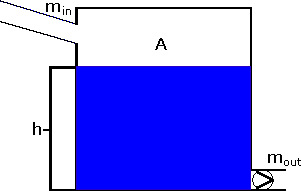
\includegraphics[width=.55\textwidth]{report/modeling/pictures/reservior.pdf}
\caption{Illustration of a tank.}
\label{fig:tank_model}
\end{figure} 

The illustration will be used to derive the model for the tank. From the left, a pipe that discharges fluid into the tank is shown. The fluid going into the tank has a mass flow rate $m_{in}$ $\left[kg/s\right]$. At the bottom right, the fluid is discharged from the tank with a mass flow rate, $m_{out}$. 
% Within the tank the stored fluid has a height, h [$m$], and the tank has a surface area, A.
Within the tank the height of the stored fluid is dependent on horizontal cross-section area and the mass in- and outflow.
%The output mass flow is dependent on the opening degree (OD) of the valve. 
The mass balance equation is derived in \cite{model_tank} and is given as:

%Assumption: incompressible flow

\begin{equation}
         \frac{dM_{cv}(t)}{dt}=m_{in}(t)-m_{o ut}(t)
\label{eq:tank_mass_balance}
\end{equation} 

Where $M_{cv}$ is the total mass within the control volume $\left[kg\right]$, and $m_{in}$ and $m_{out}$ is the mass in and outflow rate of the tank $\left[kg/s\right]$. The mass balance can be written as $M_{cv} = \rho Ah$ where $\rho$ is the density $\left[kg/m^3 \right]$, A is the area $\left[m^2\right]$ and h is the height [m]. The mass flow rate can be written as $m = \rho Q$, where Q is the flow $\left[ m^3/s \right]$. Inserting this into equation \ref{eq:tank_mass_balance} the following is obtained:

\begin{equation}
        \frac{d(\rho Ah(t))}{dt}=\rho Q_{in}(t)-\rho Q_{out}(t)
\end{equation}

By assuming incompressible fluid such that density is constant then the in- and outflow can be isolated.

\begin{equation}\label{eq:balance_reservior}
    \rho A\frac{dh(t)}{dt}=\rho \left(Q_{in}(t)-Q_{out}(t)\right)
\end{equation}
Simplifying equation \ref{eq:balance_reservior} by dividing with $\rho A$:

\begin{equation}\label{eq:balance_reserviorv2}
    \frac{dh(t)}{dt}=\frac{1}{A} \left(Q_{in}(t)-Q_{out}(t)\right)
\end{equation}

This equation describes the change in height according to in- and outflow. Due to the nature of a sewer system, it is typically not possible to implement a tank where the outflow is controlled by gravity and a valve. For this reason, it is decided to implement an actuator in the form of a pump within the tank, which control the output flow into the adjoining pipe.
In figure \ref{fig:reservior_with_pump} the chosen tank setup is seen.
%However, it has been chosen for this project to have a pump regulating the output of the tank as shown in figure \ref{fig:reservior_with_pump}.

\begin{figure}[H]
    \centering
    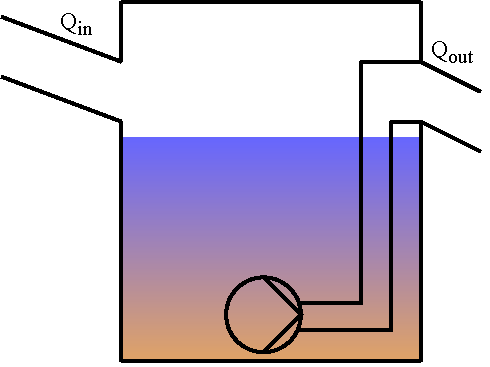
\includegraphics[width=0.55\textwidth]{report/modeling/pictures/reservior_with_pump}
    \caption{Illustration of a tank with a pump inserted to regulate the output flow.}
    \label{fig:reservior_with_pump}
\end{figure}

Due to the nature of free flow in pipes, the dynamics of the pump will be mitigated for longer pipes. For this reason, it is decided to disregard pump dynamics and implement a simple linear term where an actuator input controls the output flow.
%To simplify the model it has been chosen to use a linear pump model where the output flow, $Q_{out}$ is depended on a constant between 1 and 0 and the maximum flow that the following pipe can transfer.

\begin{equation} \label{eq:control_signal_pump_tank}
    Q_{out}(t) = u(t) \cdot \overline Q
\end{equation}
Where u is pump control input and $\overline Q$ is a fixed operating point which for example could be the maximum flow of the adjoining pipe. By inserting equation \ref{eq:control_signal_pump_tank} into equation \ref{eq:balance_reserviorv2} the following is obtained:

\begin{equation}\label{eq:final_pump_model}
 \boxed{     \frac{dh(t)}{dt}=\frac{1}{A} \left(Q_{in}(t)-u(t) \cdot \overline Q \right) }
\end{equation}

Equation \ref{eq:final_pump_model} then gives an expression where a change in height is given as a function of inflow and outflow. 

For the concentration part of the tank, there is the ratio of concentrate to consider. At some point, the level of concentrate flowing into the tank might differ from the concentrate level already in the tank. Then as the stored fluid is pumped out of the tank the concentrate level should go towards the inflow concentration. When empty the concentration of the outflow should be equal to the inflow concentration. By the initial assumptions the change in concentration in the tank is given by equation \ref{eq:prut_i_tank_equation}.

\begin{equation} \label{eq:prut_i_tank_equation}
    \frac{dC_{tank}(t)}{dt} = C_{in}(t) \cdot \frac{\frac{Q_{in}(t)}{A}}{h(t)} - C_{out}(t) \cdot \frac{\frac{Q_{out}(t)}{A}}{h(t)}   
\end{equation}

As the output concentration is equal to what is in the tank at the current time the following is obtained.

\begin{equation} \label{eq:prut_i_tank_equation2}
\boxed{    \frac{dC_{tank}(t)}{dt} = \frac{1}{A} \left(C_{in}(t) \cdot \frac{Q_{in}(t)}{h(t)} - C_{tank}(t) \cdot \frac{Q_{out}(t)}{h(t)} \right) }   
\end{equation}

The advantage of this scheme is that flow and height are already known. This keeps the computational power required at a minimum while some realism, in the level of concentrate flowing through the tank, is obtained.

% Because the output flow is depending on the OD of the valve, a model is needed to described the output flow of it. The model for the valve is derived by \cite{boysen} and is given as:
% \begin{equation}\label{eq:valve_model}
%     Q_{out} = kv(OD) \sqrt{\Delta p}
% \end{equation}
% Where kv(OD) is a function that describes the flow for different ODs. $\Delta p$ is the pressure drop across the valve [Pa]. The pressure difference across the valve is the pressure at the bottom of the tank minus the pressure in the open channel. The pressure at the bottom of the tank can be found with:
% \fxnote{Skal nok jhave noget med ventil karakterstik med}
% \begin{equation}\label{eq:pressure_at_depth}
%      P_{bot} = P_{top} +\rho g h
%  \end{equation} 
%  Where $P_{top}$ is the atmospheric pressure $[Pa]$ and g is the gravitational constant $\left[\frac{m}{s^2}\right]$. The pressure on the output side of the valve is assumed to be 1 atm as it is an open channel. Inserting equation \ref{eq:pressure_at_depth} into equation \ref{eq:valve_model} the following is obtained:    


% \begin{equation}\label{eq:valve_modelv2}
%     Q_{out} = kv(OD) \sqrt{(P_0 +\rho g h)- P_0} = kv(OD) \sqrt{\rho g h} 
% \end{equation}

% Equation \ref{eq:valve_modelv2} can be inserted into equation \ref{eq:balance_reserviorv2} and thereby the following model for the reservoir is obtained.

% \begin{equation}\label{eq:balance_reserviorv3}
%     \frac{dh(t)}{dt}=\frac{1}{A} \left(Q_{in}(t)-\left(kv(OD) \sqrt{\rho g h(t)}\right)\right)
% \end{equation}

% Equation \ref{eq:balance_reserviorv3} then gives an expression where a change in height is given as a function of inflow, pressure and an opening degree of the valve. 